\section{Αλληλεπίδραση νέφους με Jet}
	Εφόσον έχουμε κατασκευάσει το μοντέλο ενός μοριακού νέφους μπορούμε να προχωρήσουμε στη προσομοίωση της αλληλεπίδρασης ενός πλήθους τέτοιων νεφών με έναν σχετικιστικό πίδακα υλικού (που προέρχεται από το κέντρο του γαλαξία).
	
\subsection{Ορισμός του προβλήματος}
	Όπως και προηγουμένως θα ξεκινήσουμε με ένα test problem με σχετικά μικρό αριθμό νεφών ώστε να μελετήσουμε την ευστάθεια και την αποτελεσματικότητα του κώδικα.
	
\begin{marginfigure}
	\centering
	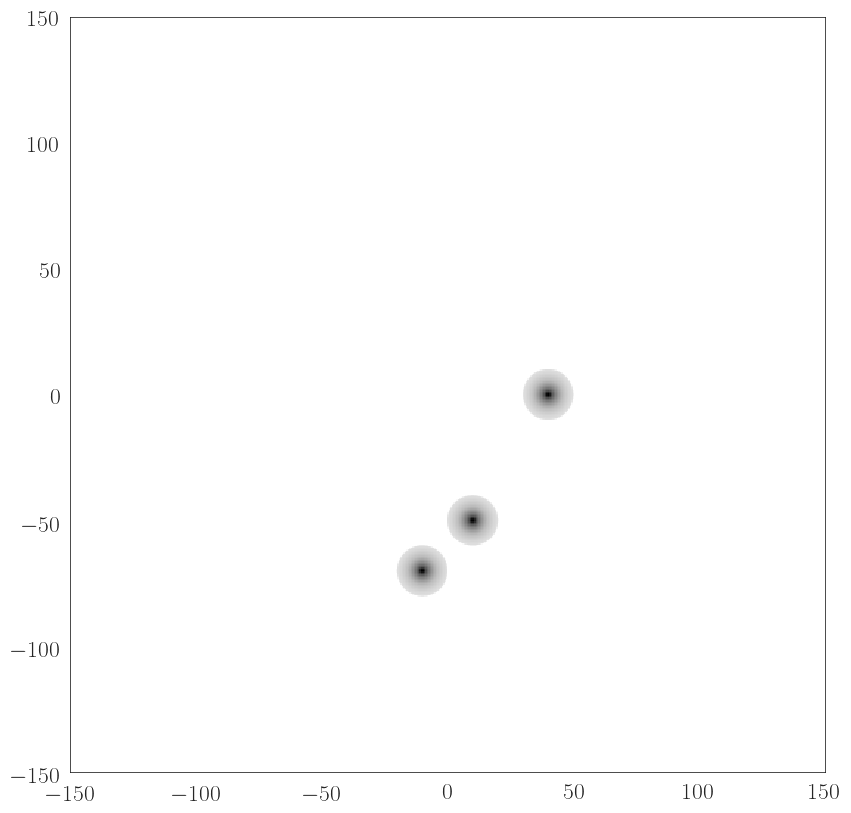
\includegraphics[width=1\linewidth]{DataImages/Jet0}
	\caption{}
	\label{fig:jet0}
\end{marginfigure}

	Έτσι ξεκινήσαμε με τη τοποθέτηση 3 μοριακών νεφών με κατανομή πυκνότητας όπως ορίστηκε στο προηγούμενο κεφάλαιο και ακτίνας \SI{10}{pc}. Τα μοριακά νέφη βρίσκονται μέσα στη μεσοαστρική ύλη με πυκνότητα \SI{1}{cm^{-3}} σε ένα τετραγωνικό χωρίο με μέγεθος \SI{300}{pc} το οποίο το χωρίζουμε σε \SI{512}{pixel}. Έτσι έχουμε μια ανάλυση των \SI{0.58}{pc}. 
	
	Για τον πίδακα χρησιμοποιούμε μια τροποποιημένη συνοριακή συνθήκη για κέντρο του κάτω σύνορο του χωρίου όπου προσδίδουμε μια σχετικιστικά ροή υλικού με πυκνότητα \SI{1e-4}{cm^{-3}} και παράγοντα lorentz $\gamma = 4$. Η διατομή της ροής είναι στα \SI{1.5}{pc}.
	
	 
	
		
